\subsection{The Orbit and the Message: From Kepler to Control}

Take \textbf{Kepler’s Second Law}: a planet sweeps out equal areas in equal times as it orbits the Sun. At first glance, it is a geometric regularity—a celestial truth extracted from Tycho Brahe’s mountain of observational data and Kepler’s extraordinary interpretive effort. It is often hailed as a victory of empiricism: a passive reading of the heavens through the patient accumulation of facts.

But Kepler’s insight carried more than geometry—it gestured toward structure, constraint, and ultimately, optimization. Beneath the law lies the conservation of angular momentum, a quantity later formalized through Newtonian mechanics and the central nature of the gravitational force. Because gravity exerts no torque about the Sun, a planet’s angular momentum remains invariant, and the sweeping of equal areas emerges as a consequence.

This classical interpretation emphasizes laws and causes: force, mass, and motion. But in the language of \textbf{optimal control theory}, particularly in Pontryagin’s Maximum Principle (PMP), Kepler’s law acquires a deeper interpretation. It ceases to be merely the byproduct of passive motion and becomes instead a \emph{necessary condition for optimality} in a system governed by symmetry.

Here lies the philosophical pivot. Control theory reframes the orbit not as a mechanical artifact but as the solution to an implicit variational problem. The planet may have no control inputs—but the structure of the system behaves \emph{as if} it were optimizing something. This is not just metaphor. If the system’s \textbf{Hamiltonian} is invariant under rotation, then, by \textbf{Noether’s theorem}, a conserved quantity must exist.\footnote{Noether’s theorem, formulated by Emmy Noether in 1915 and published in 1918, states that every differentiable symmetry of the action of a physical system corresponds to a conserved quantity. In the case of rotational symmetry, the associated conserved quantity is angular momentum. Noether’s work, originally motivated by problems in general relativity, provided a profound unification of symmetry and conservation in mathematical physics.} In Pontryagin’s formulation, this conserved quantity emerges as the \emph{costate} associated with angular displacement—none other than angular momentum itself.

Thus, what Kepler discovered geometrically and Newton justified mechanically, Pontryagin’s framework explains teleologically: as the outcome of an optimization principle. The orbit is no longer just a path—it is an answer. Not to a question posed by a force, but to a question posed by structure: how can motion preserve what symmetry forbids us to lose?

The historical arc from Kepler to Pontryagin is not merely technical—it marks a transformation in the philosophical role of mathematics. Kepler described nature’s patterns. Newton explained their causes. Pontryagin suggested that such patterns might arise from universal principles of choice, embedded in the very fabric of dynamics.

This is the control theorist’s audacity: to see even natural motion as if it were designed—not by a deity or by man, but by the internal logic of the system itself. The orbit is the solution to a problem no agent needed to ask. And in that solution is information.

Symmetry begets structure. Structure begets constraint. Constraint encodes information. In this view, Kepler’s law is not just about celestial motion; it is a \emph{message}, encrypted in planetary arcs, about the invariants the universe refuses to break. The orbit is the message, and the message is optimality.

\begin{figure}[H]
\centering
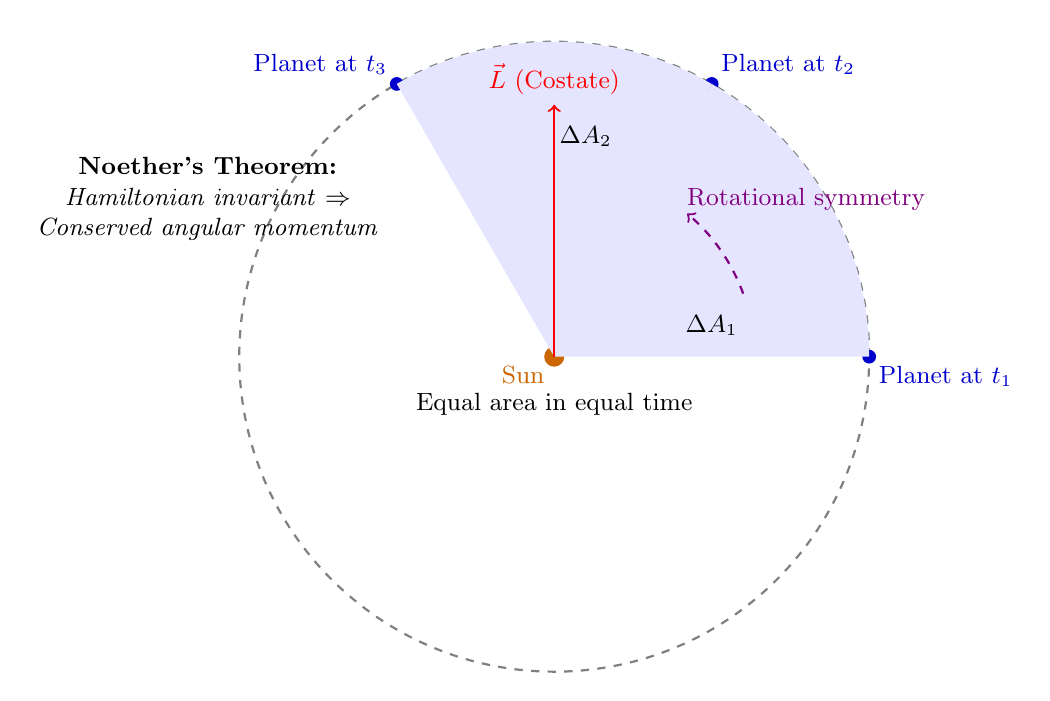
\begin{tikzpicture}[scale=4, every node/.style={font=\small}]
    % Sun
    \filldraw[orange!80!black] (0,0) circle (0.03) node[below left] {Sun};

    % Orbit path
    \draw[gray, thick, dashed] (0,0) circle (1);

    % Planet positions
    \coordinate (P1) at (1,0);
    \coordinate (P2) at ({cos(60)},{sin(60)});
    \coordinate (P3) at ({cos(120)},{sin(120)});
    
    \filldraw[blue!80!black] (P1) circle (0.02) node[below right] {Planet at $t_1$};
    \filldraw[blue!80!black] (P2) circle (0.02) node[above right] {Planet at $t_2$};
    \filldraw[blue!80!black] (P3) circle (0.02) node[above left] {Planet at $t_3$};

    % Swept areas (two sectors)
    \fill[blue!10] (0,0) -- (P1) arc (0:60:1) -- cycle;
    \fill[blue!10] (0,0) -- (P2) arc (60:120:1) -- cycle;

    % Angular momentum vector
    \draw[->, thick, red] (0,0) -- (0,0.8) node[above] {$\vec{L}$ (Costate)};

    % Equal area labels
    \node at (0.5,0.1) {$\Delta A_1$};
    \node at (0.1,0.7) {$\Delta A_2$};
    \node at (0.0,-0.15) {Equal area in equal time};

    % Rotational symmetry arc
    \draw[->, thick, violet, dashed] (0.6,0.2) arc (20:50:0.6);
    \node[violet] at (0.8,0.5) {Rotational symmetry};

    % Hamiltonian symmetry note
    \node[align=center] at (-1.1,0.5) {
        \textbf{Noether’s Theorem:}\\
        \textit{Hamiltonian invariant} $\Rightarrow$\\
        \textit{Conserved angular momentum}
    };

\end{tikzpicture}
\caption{Kepler’s Second Law interpreted through control theory: the conservation of angular momentum as a costate, the rotational symmetry of the Hamiltonian, and equal areas swept out in equal times.}
\end{figure}

\begin{table}[H]
\vspace{1.5em} % Space above the table
\centering
\renewcommand{\arraystretch}{2.0} % Even more row height
\begin{tabular}{>{\raggedright\arraybackslash}p{0.45\linewidth} | >{\raggedright\arraybackslash}p{0.45\linewidth}}
\toprule
\addlinespace[1.2em]
\textbf{Classical Newtonian Mechanics} & \textbf{Optimal Control Theory (Pontryagin)} \\
\addlinespace[1.2em]
\midrule
\addlinespace[1.2em]

\textbf{Framework:} Newton's laws, force-based dynamics &
\textbf{Framework:} Pontryagin's Maximum Principle, costate dynamics \\
\addlinespace[1.2em]

Gravitational force is central: $\vec{F} = -\frac{GMm}{r^2} \hat{r}$ &
Hamiltonian $H(x, \lambda)$ is invariant under rotation \\
\addlinespace[1.2em]

Zero torque: $\vec{\tau} = \vec{r} \times \vec{F} = 0$ &
By Noether’s theorem, symmetry $\Rightarrow$ conserved quantity \\
\addlinespace[1.2em]

Conservation of angular momentum: $\vec{L} = \vec{r} \times \vec{p}$ &
Conservation of costate: $\lambda_\theta = \text{const}$ (angular momentum as costate) \\
\addlinespace[1.2em]

Area swept: $\frac{dA}{dt} = \frac{1}{2} r^2 \frac{d\theta}{dt}$ &
Costate conservation implies $\frac{dA}{dt} = \text{const}$ \\
\addlinespace[1.2em]

\textit{Equal areas in equal times} is a geometric result &
\textit{Equal areas in equal times} is a necessary condition for optimality \\
\addlinespace[1.2em]

\textbf{Conclusion:} Result of torque-free motion under a central force &
\textbf{Conclusion:} A structural constraint from rotational symmetry in Hamiltonian \\
\addlinespace[1.2em]
\bottomrule
\end{tabular}
\vspace{1.5em} % Space below the table
\caption{Comparison of Kepler’s Second Law under classical mechanics and optimal control theory. Both yield conservation of angular momentum, but through distinct interpretive frameworks.}
\end{table}
